\documentclass[journal,12pt,twocolumn]{IEEEtran}
%
\usepackage{setspace}
\usepackage{gensymb}
%\doublespacing
\singlespacing

%\usepackage{graphicx}
%\usepackage{amssymb}
%\usepackage{relsize}
\usepackage[cmex10]{amsmath}
%\usepackage{amsthm}
%\interdisplaylinepenalty=2500
%\savesymbol{iint}
%\usepackage{txfonts}
%\restoresymbol{TXF}{iint}
%\usepackage{wasysym}
\usepackage{amsthm}
%\usepackage{iithtlc}
\usepackage{mathrsfs}
\usepackage{txfonts}
\usepackage{stfloats}
\usepackage{bm}
\usepackage{cite}
\usepackage{cases}
\usepackage{subfig}
%\usepackage{xtab}
\usepackage{longtable}
\usepackage{multirow}
%\usepackage{algorithm}
%\usepackage{algpseudocode}
\usepackage{enumitem}
\usepackage{mathtools}
\usepackage{steinmetz}
\usepackage{tikz}
\usepackage{circuitikz}
\usepackage{verbatim}
\usepackage{tfrupee}
\usepackage[breaklinks=true]{hyperref}
%\usepackage{stmaryrd}
\usepackage{tkz-euclide} % loads  TikZ and tkz-base
%\usetkzobj{all}
\usetikzlibrary{calc,math}
\usepackage{listings}
    \usepackage{color}                                            %%
    \usepackage{array}                                            %%
    \usepackage{longtable}                                        %%
    \usepackage{calc}                                             %%
    \usepackage{multirow}                                         %%
    \usepackage{hhline}                                           %%
    \usepackage{ifthen}                                           %%
  %optionally (for landscape tables embedded in another document): %%
    \usepackage{lscape}     
\usepackage{multicol}
\usepackage{chngcntr}
%\usepackage{enumerate}

%\usepackage{wasysym}
%\newcounter{MYtempeqncnt}
\DeclareMathOperator*{\Res}{Res}
%\renewcommand{\baselinestretch}{2}
\renewcommand\thesection{\arabic{section}}
\renewcommand\thesubsection{\thesection.\arabic{subsection}}
\renewcommand\thesubsubsection{\thesubsection.\arabic{subsubsection}}

\renewcommand\thesectiondis{\arabic{section}}
\renewcommand\thesubsectiondis{\thesectiondis.\arabic{subsection}}
\renewcommand\thesubsubsectiondis{\thesubsectiondis.\arabic{subsubsection}}

% correct bad hyphenation here
\hyphenation{op-tical net-works semi-conduc-tor}
\def\inputGnumericTable{}                                 %%

\lstset{
%language=C,
frame=single, 
breaklines=true,
columns=fullflexible
}
%\lstset{
%language=tex,
%frame=single, 
%breaklines=true
%}

\begin{document}
%


\newtheorem{theorem}{Theorem}[section]
\newtheorem{problem}{Problem}
\newtheorem{proposition}{Proposition}[section]
\newtheorem{lemma}{Lemma}[section]
\newtheorem{corollary}[theorem]{Corollary}
\newtheorem{example}{Example}[section]
\newtheorem{definition}[problem]{Definition}
%\newtheorem{thm}{Theorem}[section] 
%\newtheorem{defn}[thm]{Definition}
%\newtheorem{algorithm}{Algorithm}[section]
%\newtheorem{cor}{Corollary}
\newcommand{\BEQA}{\begin{eqnarray}}
\newcommand{\EEQA}{\end{eqnarray}}
\newcommand{\define}{\stackrel{\triangle}{=}}
\bibliographystyle{IEEEtran}
%\bibliographystyle{ieeetr}
\providecommand{\mbf}{\mathbf}
\providecommand{\pr}[1]{\ensuremath{\Pr\left(#1\right)}}
\providecommand{\qfunc}[1]{\ensuremath{Q\left(#1\right)}}
\providecommand{\sbrak}[1]{\ensuremath{{}\left[#1\right]}}
\providecommand{\lsbrak}[1]{\ensuremath{{}\left[#1\right.}}
\providecommand{\rsbrak}[1]{\ensuremath{{}\left.#1\right]}}
\providecommand{\brak}[1]{\ensuremath{\left(#1\right)}}
\providecommand{\lbrak}[1]{\ensuremath{\left(#1\right.}}
\providecommand{\rbrak}[1]{\ensuremath{\left.#1\right)}}
\providecommand{\cbrak}[1]{\ensuremath{\left\{#1\right\}}}
\providecommand{\lcbrak}[1]{\ensuremath{\left\{#1\right.}}
\providecommand{\rcbrak}[1]{\ensuremath{\left.#1\right\}}}
\theoremstyle{remark}
\newtheorem{rem}{Remark}
\newcommand{\sgn}{\mathop{\mathrm{sgn}}}
\providecommand{\abs}[1]{\left\vert#1\right\vert}
\providecommand{\res}[1]{\Res\displaylimits_{#1}} 
\providecommand{\norm}[1]{\left\lVert#1\right\rVert}
%\providecommand{\norm}[1]{\lVert#1\rVert}
\providecommand{\mtx}[1]{\mathbf{#1}}
\providecommand{\mean}[1]{E\left[ #1 \right]}
\providecommand{\fourier}{\overset{\mathcal{F}}{ \rightleftharpoons}}
%\providecommand{\hilbert}{\overset{\mathcal{H}}{ \rightleftharpoons}}
\providecommand{\system}{\overset{\mathcal{H}}{ \longleftrightarrow}}
	%\newcommand{\solution}[2]{\textbf{Solution:}{#1}}
\newcommand{\solution}{\noindent \textbf{Solution: }}
\newcommand{\cosec}{\,\text{cosec}\,}
\providecommand{\dec}[2]{\ensuremath{\overset{#1}{\underset{#2}{\gtrless}}}}
\newcommand{\myvec}[1]{\ensuremath{\begin{pmatrix}#1\end{pmatrix}}}
\newcommand{\mydet}[1]{\ensuremath{\begin{vmatrix}#1\end{vmatrix}}}
%\numberwithin{equation}{section}
\numberwithin{equation}{subsection}
%\numberwithin{problem}{section}
%\numberwithin{definition}{section}
\makeatletter
\@addtoreset{figure}{problem}
\makeatother
\let\StandardTheFigure\thefigure
\let\vec\mathbf
%\renewcommand{\thefigure}{\theproblem.\arabic{figure}}
\renewcommand{\thefigure}{\theproblem}
%\setlist[enumerate,1]{before=\renewcommand\theequation{\theenumi.\arabic{equation}}
%\counterwithin{equation}{enumi}
%\renewcommand{\theequation}{\arabic{subsection}.\arabic{equation}}
\def\putbox#1#2#3{\makebox[0in][l]{\makebox[#1][l]{}\raisebox{\baselineskip}[0in][0in]{\raisebox{#2}[0in][0in]{#3}}}}
     \def\rightbox#1{\makebox[0in][r]{#1}}
     \def\centbox#1{\makebox[0in]{#1}}
     \def\topbox#1{\raisebox{-\baselineskip}[0in][0in]{#1}}
     \def\midbox#1{\raisebox{-0.5\baselineskip}[0in][0in]{#1}}
\vspace{3cm}
\title{Assignment 9.10.5.11}
\author{Shristy Sharma (EE22BNITS11001)}
% make the title area
\maketitle
\newpage
%\tableofcontents
\bigskip
\renewcommand{\thefigure}{\theenumi}
\renewcommand{\thetable}{\theenumi}
%\renewcommand{\theequation}{\theenumi}
\section{Problem}
ABC and ADC are two right triangles with common hypotenuse AC. Prove that
$\angle CAD$ = $\angle CBD$.
\section{Solution}
We will use vectors to prove that $\angle CAD = \angle CBD$. \\
Let's assume that A, B, C, and D are the vertices of the two right triangles.\\
We can represent the position vectors of points A, B, C, and D as $\vec{a}, \vec{b}, \vec{c}, and \vec{d},$ respectively. Then we have:
\begin{align}
\vec{AB} &= \vec{b} - \vec{a}\\
\vec{AC} &= \vec{c} - \vec{a}\\
\vec{CD} &= \vec{d} - \vec{c}
\end{align}
Since ABC and ADC are right triangles, we know that:
\begin{align}
\vec{AB} \cdot \vec{AC} &= 0 \\
\vec{CD} \cdot \vec{AC} &= 0 
\end{align}
Taking the dot product of (2.0.4) with (2.0.5), we get:
\begin{align}
\vec{AB} \cdot \vec{AC} \cdot \vec{CD} \cdot \vec{AC} &= 0\\
\vec{AB} \cdot \vec{AC} \cdot (\vec{d} - \vec{c}) \cdot \vec{AC} &= 0\\
(\vec{AB} \cdot \vec{AC}) \vec{d} \cdot \vec{AC} - (\vec{AB} \cdot \vec{AC})\vec{c} \cdot \vec{AC} &= 0
\end{align}
Since AC is non-zero, we can divide both sides by $\norm {\vec{AC}}^2$ to get:
\begin{align}
\brak{\vec{AB} \cdot \vec{AC}} \brak{ \frac{\vec{d} \cdot \vec{AC}} {\norm {\vec{AC}}^2 } }- \brak{\vec{AB} \cdot \vec{AC} }\brak{\frac{\vec{c} \cdot \vec{AC}} {\norm {\vec{AC}}^2 } } = 0
\end{align}
But $\frac { \vec{d} \cdot \vec{AC}} {\norm {\vec{AC}}^2} = \cos \angle CAD $ and $\frac{\vec{c} \cdot \vec{AC}} {\norm {\vec{AC}}^2}= \cos \angle CBD$. Therefore, we have:
\begin{align}
\brak{\vec{AB} \cdot \vec{AC}}\cos\angle CAD - \brak{\vec{AB} \cdot \vec{AC}}\cos\angle CBD &= 0\\
\brak{\vec{AB} \cdot \vec{AC}} \brak{\cos\angle CAD - \cos\angle CBD} &= 0\\
\vec{AB} \cdot \vec{AC} &= 0
\end{align}
Since $\vec{AB}$ and $\vec{AC}$ are non-zero and $\cos\angle CAD - \cos \angle CBD$ cannot be zero, we conclude that $\vec{AB} . \vec{AC}$ must be zero. Therefore, we have:
\begin{align}
\brak{\vec{b} - \vec{a}} \cdot \brak{\vec{c} - \vec{a}} &= 0
\end{align}
Since AB and AC are orthogonal, and CD and AC are also orthogonal, we can conclude that AB and CD are parallel:
\begin{align}
\vec{AB} \perp \vec{AC}\\
\vec{CD} \cdot \vec{AC} &= (\vec{d} - \vec{c}) \cdot (\vec{c} - \vec{a}) = 0\\
\vec{CD} \perp \vec{AC}\\
\vec{AB} \times \vec{AC} &= (\vec{b} - \vec{a}) \times (\vec{c} - \vec{a}) = 0\\
\vec{CD} \times \vec{AC} &= (\vec{d} - \vec{c}) \times (\vec{c} - \vec{a}) = 0
\end{align}
Therefore, the two right triangles ABC and ADC are similar, and we have:
\begin{align}
\angle CAD &= \angle ACD = \angle CBD\
\end{align}
\begin{figure}[h!]
  \centering
   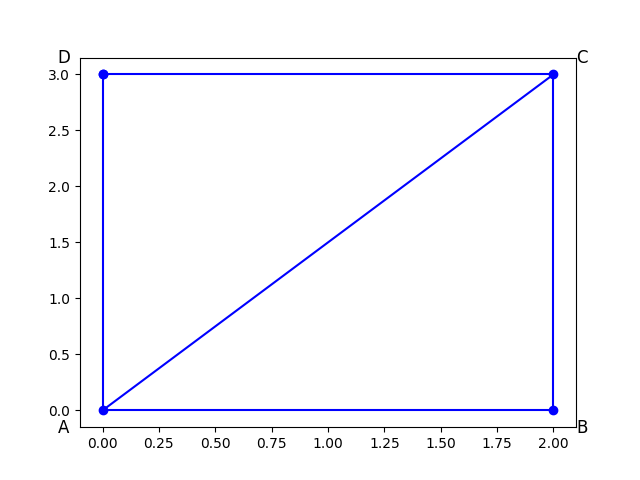
\includegraphics[width=\columnwidth]{figs/fig_1.png}
    \caption{Plot of $ABCD$}
     \label{fig:1}  
\end{figure}
\end{document}